\documentclass{acmsiggraph}               % final
%\documentclass[review]{acmsiggraph}      % review
%\documentclass[widereview]{acmsiggraph}  % wide-spaced review
%\documentclass[preprint]{acmsiggraph}    % preprint

%% Uncomment one of the four lines above depending on where your paper is
%% in the conference process. ``review'' and ``widereview'' are for review
%% submission, ``preprint'' is for pre-publication, and ``final'' is for
%% the version to be printed.

%% These two line bring in essential packages: ``mathptmx'' for Type 1 
%% typefaces, and ``graphicx'' for inclusion of EPS figures.

\usepackage{mathptmx}
\usepackage{graphicx}

%% use this for zero \parindent and non-zero \parskip, intelligently.

\usepackage{parskip}
\usepackage{subfigure}
\usepackage{smrdefaults}

%% If you are submitting a paper to the annual conference, please replace 
%% the value ``0'' below with your OnlineID. If you are not submitting this
%% paper to the annual conference, you may safely leave it at ``0'' -- it 
%% will not be included in the output.

\onlineid{0}

%% need to document this!

\acmformat{print}

%% Paper title.

\title{Sound Texture Synthesis\\(revision 2)}

%% Author and Affiliation (single author).

\author{Ananya Misra, Perry R. Cook, and Ge Wang\\Princeton University\thanks{e-mail: \{amisra, prc, gewang\}@cs.princeton.edu}}

%% Author and Affiliation (multiple authors).

%%\author{Roy G. Biv\thanks{e-mail: roy.g.biv@aol.com}\\ Starbucks Research %
%%\and Ed Grimley\thanks{e-mail:ed.grimley@aol.com}\\ Grimley Widgets, Inc. %
%%\and Martha Stewart\thanks{e-mail:martha.stewart@marthastewart.com}\\ Martha Stewart Enterprises \\ Microsoft Research}

%% Keywords that describe your work.

\keywords{sound texture, synthesis, sinusoidal modeling, wavelet}

%%%%%% START OF THE PAPER %%%%%%

\begin{document}

\teaser{
  \subfigure[original]{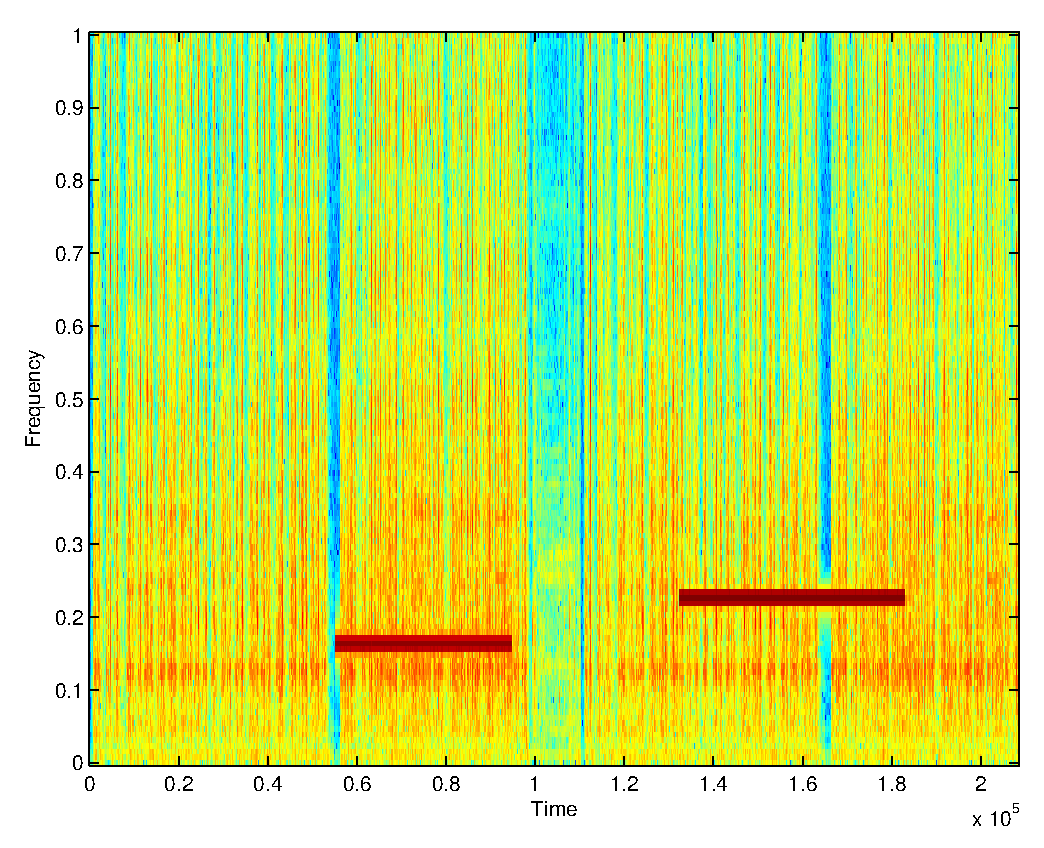
\includegraphics[width=.24\textwidth]{story1.eps}}
  \subfigure[foreground]{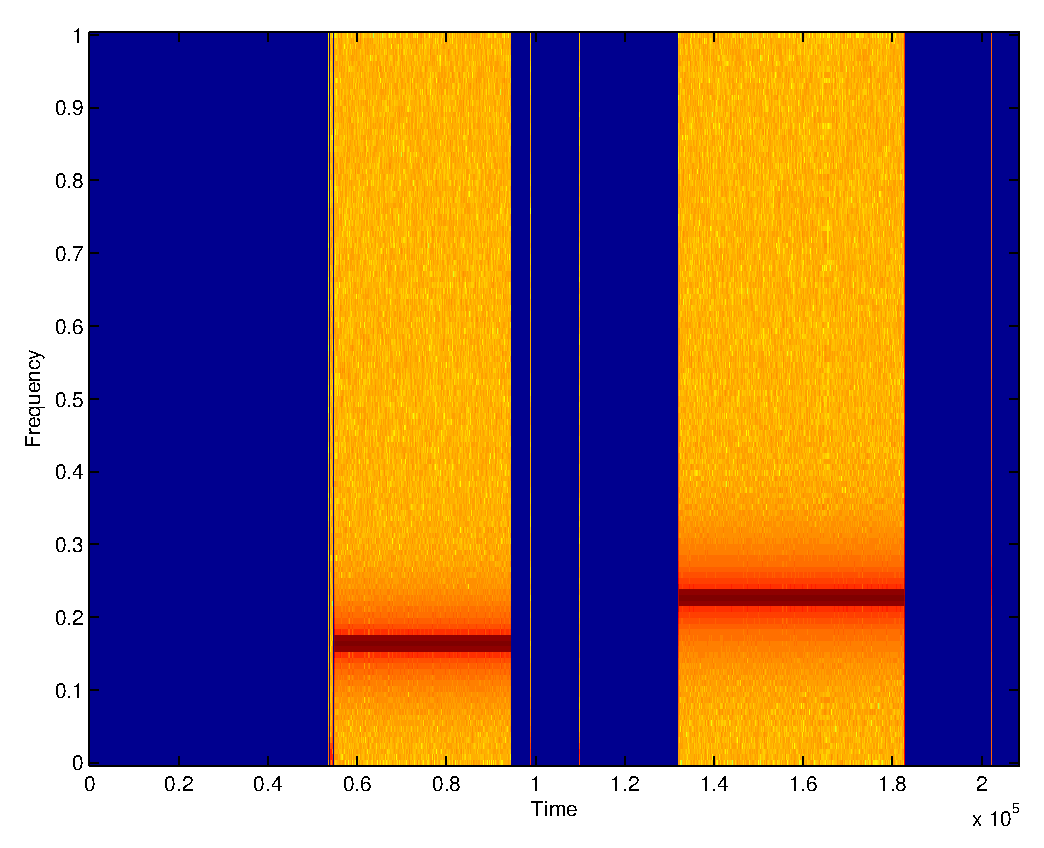
\includegraphics[width=.24\textwidth]{story2.eps}}
  \subfigure[background]{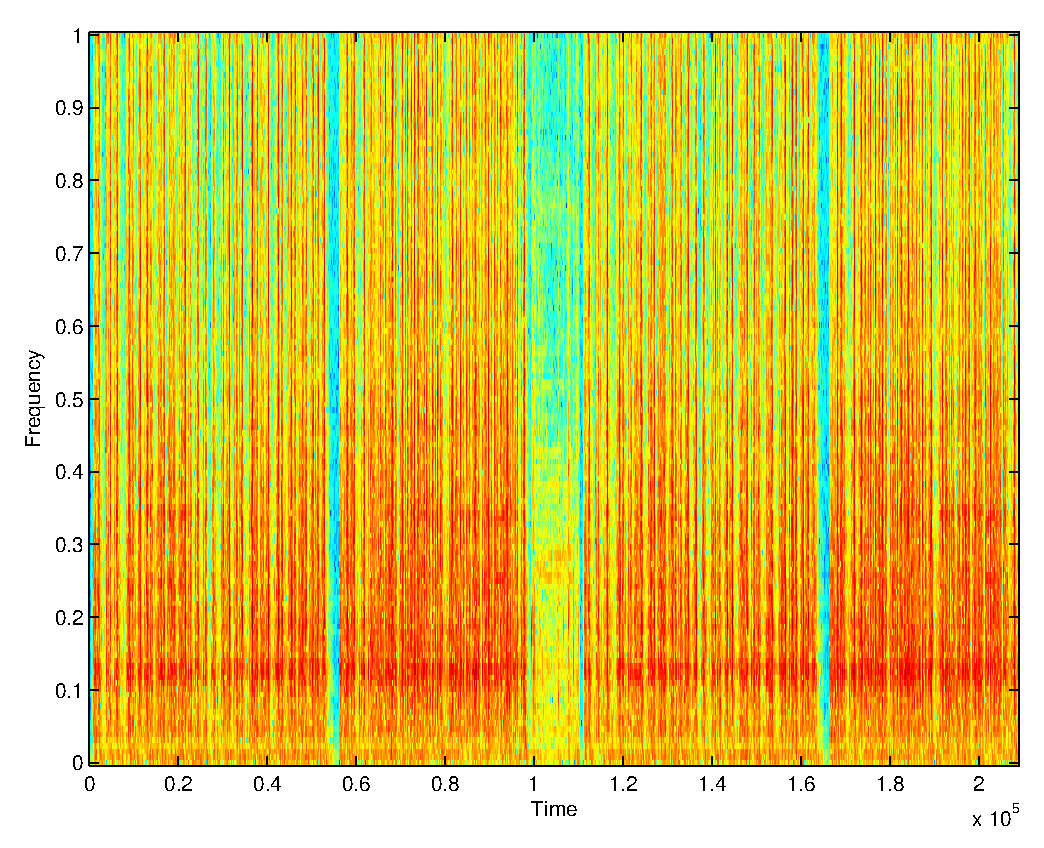
\includegraphics[width=.24\textwidth]{story3_fake.eps}}
  \subfigure[synthesized]{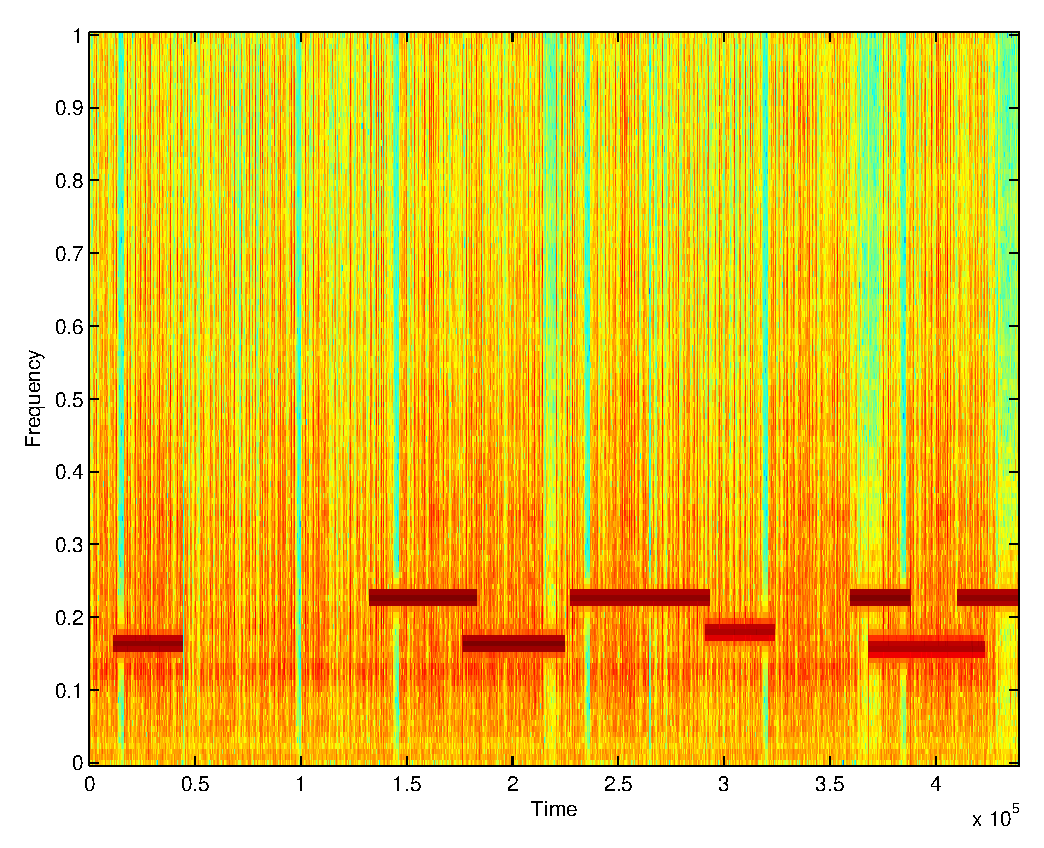
\includegraphics[width=.24\textwidth]{story4_fake.eps}}
  \caption{The original sound texture (a) is separated into deterministic foreground events 
(b) and stochastic background texture (c).  A new texture (d) is generated. }
}

% The ``\maketitle'' command must be the first command after the
% ``\begin{document}'' command. It prepares and prints the title block.

\maketitle

% Abstract section.

\begin{abstract}

%This paper is abstract (in many ways).
`
We describe a framework for synthesizing perceptually-convincing sound textures of unlimited 
length, with fine control over the characteristics and occurrences of individual foreground events
and the qualities of the background sound.  Given an 
example texture, the system can automatically locate and isolate sinusoidal events, transient
events, and background textures into reusable templates.  Our framework also allows users 
to interactively highlight points of interest in the sound for event isolation, manipulate events independently, change the density of events, and even create new sound textures by combining elements of different source templates.  

Our general approach models foreground events and background sound separately. We apply 
spectral modeling to extract sinusoidal or deterministic events and a stochastic residue from the given sound.  The deterministic events are then generated to order, possibly after spectral transformations, 
using sinusoidal resynthesis. The stochastic component may also contain non-sinusoidal events, 
known as \textit{transients}. We generate the stochastic component using wavelet tree learning. The 
resulting system provides a new paradigm for interactively synthesizing high-quality sound 
texture with flexible control over the variety and quality of the synthesized sound.


%Citations can be done this way~\cite{Jobs95} or this more concise 
%way~\shortcite{Jobs95}, depending upon the application.
\end{abstract}

% ACM Computing Review (CR) categories. 
% See <http://www.acm.org/class/1998/> for details.
% The ``\CRcat'' command takes four arguments.

%\begin{CRcatlist}
%  \CRcat{K.6.1}{Management of Computing and Information Systems}%
%{Project and People Management}{Life Cycle};
%  \CRcat{K.7.m}{The Computing Profession}{Miscellaneous}{Ethics}
%\end{CRcatlist}

% The ``\keywordlist'' command prints out the keywords.
\keywordlist

\section{Introduction}
% The ``\copyrightspace'' command must be the first command after the 
% start of the first section of the body of your paper. It ensures the
% copyright space is left at the bottom of the first column on the first
% page of your paper.
\copyrightspace
Many sound synthesis techniques focus on generating foreground sounds such as voices, music or 
sudden events that easily hit the ear. These sounds alone do not generally give the listener a 
strong sense of being in a real-world environment where there are many background noises as 
well. The totality of sounds that compose an auditory environment are an example of sound 
textures.

A sound texture can be described as a sound with structural elements that repeat over time, 
but with some randomness. The randomness prevents it from being modeled well by strictly 
deterministic techniques. On the other hand, the sound cannot be modeled as a purely random 
process since on some level it appears stationary, or has an almost stable structure.

Sound texture synthesis is the creation of perceptually convincing sound based on a set of 
example sounds. The generated sound should be sufficiently like the original to be perceived 
as another instance of it. However, merely repeatedly playing the original sound is not 
convincing, so the synthesis should also involve some randomness. 

Given one or more example sound textures, we would like to generate from these an unlimited 
supply of non-repeating, perceptually convincing sound that can be parametrically controlled 
to fit the user's specifications. One of our goals is to give sound designers for 
entertainment (movies, TV, and games), Virtual and Augmented Reality, and art projects such as 
live performance and installations, an automation tool for easily modeling and generating 
sound textures.

Our general approach is based on the notion that sound textures are composed of events as well 
as background sound, which are best modeled separately. We apply spectral modeling 
~\cite{Serra89} to extract sinusoidal or deterministic events and a stochastic residue from 
the given sound. The deterministic events are then generated to order, possibly after spectral 
transformations, using sinusoidal resynthesis. The stochastic component may also contain 
non-sinusoidal events, known as transients. We generate the stochastic component using a 
wavelet tree learning algorithm by Dubnov et. al. ~\shortcite{Dubnov02}. Feeding it the 
residue, with no sinusoidals or harmonic events, allows the wavelet tree learning to operate 
on the type of data with which it works best.  SMS techniques has been primarily used for 
analysis/modeling of foreground musical sounds.  We are the first (and the last probably) to 
use it for event separation in texture synthesis.

Our method also allows users to have control over the characteristics of their synthesized 
texture. Separating the events provides a framework in which to manipulate events 
individually, and to request more occurences of some events and less of others in the final 
texture. It also offers the option or creating new sound textures by mixing the backgrounds 
and deterministic events from several example textures.

%PLACEHOLDER: our contributions are too numerous to list here, a random sampling:
% observation: separation of foreground events and background din is beneficial
%    - indepedently transform events and background
%    - you can add or remove instances of events
%    - mix events from different sources
%    - better results (we hope) from wavelet
% contribution:
%    - system for doing it
%    - a user interface for building new sound textures

%   1.1 Motivation\\
%   		 - what is a sound texture anyway?\\
%       - "i have this sound texture, I want to produce more of it.
%          and in this way (clarifify)"\\
%       - give sound designers automation tool\\
%   1.2 Our general approach (what we are describing in this paper)\\
%	- we like wavelet tree learning and we like sms\\
%	- we want to realize the future section of wavelet tree, be able to point at 
%components of a sound and ask for more or less of it\\
%	- using sms plus feature based audio classification we gain\\
%	---we can separate out events/foreground\\
%	---we make wavelet tree better because we separate harmonic events, which wavelet tree 
%is not good at handling\\
%	- transform: because we have individual events we can modify and place them 
%independently\\
%	- more control over the textures we synthesize (example somewhere)\\

\section{Related Work}

Previous work on synthesizing sound to match a given environment has 
involved simulation or model-based methods for generating interactive 
contact sounds, or the analysis and resynthesis of existing sounds. 
While our work draws on ideas from the former, we focus more on the 
analysis and resynthesis of environmental sounds.

%         - perry's book
         
\subsection{Simulated and Model-based Sounds}

Interactive contact sounds such as scraping, rolling and walking have 
been synthesized by modeling the physics or spectrum of the sound source.

The FOLEYAUTOMATIC software system by Doel et. al. ~\shortcite{Doel01} uses dynamic simulation 
with a modal audio model based on contact forces and a graphics renderer to create interactive 
simulations with high-quality audio. 

In the Sounding Object project by Rocchesso et. al. ~\shortcite{Rocchesso03}, physically based 
models are applied to generate complex sounds. 

%       - interactive (contact) sounds\\
%         --- foley automatic (2001)\\
%         --- sounding objects\\
%         --- bill's gait (2002)\\
%         --- dinesh pai\\
%         --- doel\\
%       - motion-driven synthesis\\
%       - aerodynamic sound (transition into next subsection?)\\

A related area is perceptual rendering, where the sound sources 
correspond to actual entities in the virtual environment. They are 
manipulated or combined based on the listener's position in the model. 
Tsingos et. al. ~\shortcite{Tsingos04} demonstrated a method to 
efficiently render many (hundreds of) moving sound sources, using 
auditory culling and spatial clustering. 

The advantage of this approach is that sound can be
directly infered/synthesized, given a model.  sounds can
be "intuitively" modified by modifying the model. The
downside is that you need a model in order to generate
sound so it's hard to generalize.

%this is not what we are doing.

\subsection{Environmental Sounds}

The ultimate goal in sound texture synthesis is to generate an unlimited 
supply of non-repeating, perceptually convincing, parametrically controlled sound, based on a 
given set of example sound clips. This method assumes no prior knowledge of the geometry of, 
or the objects in, a particular environment.

Existing work includes various ways of analyzing, transforming and 
resynthesizing the source sound. 

Athineos and Ellis ~\shortcite{Athineos03} used cascading time-frequency 
linear prediction (CTFLP) to model very brief granular events known as 
\textit{micro-transients}. Examples include fire crackling, people applauding, or 
soda being poured out of a bottle. Performing linear prediction in both the time and frequency 
domains captured these sounds that normal time-domain linear prediction misses. 
%While this 
%method is effective, it was designed for a specific type of noisy 
%texture and also generates an output texture of the same length as the 
%source sound.
This method is effective on textures that primarily contain micro-transients, but does not
generalize well to other sounds and the output texture is limited to the same length as the 
source sound.

Zhu and Wyse ~\shortcite{Zhu04} extended the cascading time-frequency 
linear prediction technique and applied it to separate the foreground 
transient sequence from the background din in the source texture. Their 
method performs a frame-based CTFLP analysis and observes the change in the gain of the 
time-domain linear prediction across frames to detect events. It then segments these 
out to obtain a background. A background sound of the desired length is generated using a 
noise excited time-domain linear predictive filter, while events are generated using the CTFLP 
method on clusters of the CTFLP coefficients. The background and events are then combined to 
obtain the final texture. However, this method does not take frequency into account while 
identifying events, and hence does not distinguish spectral events. Moreover, since it extends 
CTFLP, its effectiveness is also limited to sound containing mostly micro-transients.

Miner and Caudell ~\shortcite{Miner97} used wavelets to decompose, transform or modify,
and resynthesize various background sound textures including rain, wind, crackling fire, etc. 
Their work concentrated on the perceptual effects of various transformations.
%Miner and Caudell ~\shortcite{Miner97} used wavelets to synthesize stochastic-based sounds. 
%They classified stochastic sounds into two classes: continuous sounds such as wind, rain and 
%sliding, and impact sounds such as a door knock or glass breaking. 
The use of wavelets 
instead 
of the Fourier transform allowed them to model the time varying nature of the sounds, since 
it 
provided variable-sized time windows for studying information at variable frequencies. With 
this method, they showed that the wavelet coefficients at different frequencies could be 
manipulated to alter the sound. 
The parameters to be manipulated did 
not directly map to the audible characteristics of the resulting sound, so some high-level 
knowledge was required for obtaining specific results. Also although this was a method for 
transforming sound, it didn't generate more of a texture. 

Dubnov et. al. ~\shortcite{Dubnov02} also used a wavelet decomposition to 
analyze the temporal and spectral structure of a sound texture at various 
resolutions. Treating the input sound texture as a sample of a stochastic process, 
they performed stochastic learning to generate wavelet coefficients for the synthesized 
texture. The synthesized texture could be controllably close to the source by some measure of 
error. This technique focused on generating a sound texture close to the original rather than 
on transforming the original sound texture. The results were best for sounds with periodic or 
pitched components of short duration, and for mostly stochastic sounds. However, synthesizing 
mixtures of stochastic and continuous pitched sounds, or periodic sounds of strong temporal 
coherence in this way sometimes resulted in the undesirable chopping up of continuous sounds. This 
happened due to the small amount of randomness permitted in learning the wavelet coefficients. 
Even though this measure of error could be controlled, setting it to an extremely low value 
produced sound textures almost exactly identical, temporally as well as spectrally, to the 
original.

These existing approaches do not allow much control over the output - either the entire texture
is transformed (Miner et. al) or segments are shuffled and concatenated blindly. There's an extra
dimension that they don't take care of, and that's different events happening simultaneously.
For example, \textit{what example?}
%In all of the existing approaches, the final output is limited by the original "mixture" of
%the source sound - no (new) densities or combinations of sounds can be constructed without
%actually being present in the orginal
Our approach overcomes these limitations by isolating pitched sounds, performing wavelet tree 
learning on the remaining stochastic part, and re-inserting the pitched components afterwards. 
We separate the pitched components from the sound texture using spectral modeling.


%Given an existing ambient/background/environment sound of limited, 
%length, it is possible to synthesize more of the same texture. This 
%method has no prior knowledge of the objects in the environment. 


%       - texture synthesis from existing ambient/background/environment
%         sounds (of limited length)\\
%       - LPC fails (probably)\\
%         --- good for micro-transients\\
%       - dubnov et. al.  (2002)\\
%         --- showed how to take apart and synthesize more of it but...\\
%         --- individual events not good for chopping up, not good for repeating\\
%       - miner and caudell\\
%       - we come in here...\\
%         --- event identification/isolation/transformation/(authentification)
%           (better analysis)\\
%         --- take better advantage of wavelet tree learning \\
%         --- separation of control over background and events
%           (more control during synthesis)\\
%         --- more potential for interactivity\\
%         --- combine many of these approachs + spectral modeling\\
%         --- talk about how our stuff differs\\

\subsection{Spectral Modeling}

Spectral modeling builds on the notion that some components of sound fit a sinusoidal model 
while others are modeled better by spectrally shaped noise. The Fourier transform allows us to 
observe the spectrum of a sound and identify the components that would best be modeled by 
sinusoids. These are also known as the deterministic components of the sound. We can then 
subtract these components from the original sound and ideally end with only the noise 
component, also called the residual or stochastic component. 

Xavier Serra and Julius Smith ~\shortcite{Serra89} posed and implemented the concept of "sines 
plus noise" modeling in the Spectral Modeling Synthesis (SMS) system. The SMS system also 
offers options for modifying the original sound before resynthesis, for instance by 
pitch-shifting and time-stretching.

Thornburg and Leistikow ~\shortcite{Thornburg03} developed a hybrid state-space sinusoidal 
model that uses an iterative filterbank to split the sound into subbands. In each subband, the 
instantaneous sinusoidal phase and frequency are estimated and the latter is used to set 
parameters for the next iteration. They employed this method for modeling signals that are 
"quasi-harmonic", with a loose harmonic structure and some possible inharmonicity. 

Traditional methods for obtaining a signal's spectrum often assume that the data is stationary 
and has uniform spacing between samples. This is not always the case for real data. Qi et. al. 
~\shortcite{Qi02} address this by using a non-stationary Kalman filter within a Bayesian 
framework to estimate spectral coefficients. 

%\begin{equation}
% \sum_{j=1}^{z} j = \frac{z(z+1)}{2}
%\end{equation}

\section{Overview of our Approach}

To demonstrate how the system works, we give an example that begins with 
an existing sound texture, and shows the stages involved in generating new 
sounds textures.    While the system can operated unsupervised from 
beginning to end (given a set of parameters), it is possible to interact 
with it at various points in the pipeline.  We will highlight the control 
points and the parameters as appropriate.

The system starts with an existing sound texture, which we will refer to as the
\textit{template}.  An example template may be the sound of a city street, a factory 
environment, seagulls by the ocean, a sporting event, or anything other
ambient or semi-ambient sound.  The duration of 
the template may be around 30-45 seconds or more, depending on the
contents of the sound.  Sound events in the street template, for example, 
may include (1) car horns, (2) screeching of vehicle brakes, (3) engines accelerating 
(4) cars passing by with dopplar shift, (5) engines starting, and (6) random
bangs and pops.  Background textures might include indistinct chatter of pedestrians
and the general hum/din of the surrounding/city.

No \textit{a priori} knowledge about the existing sound is necessary, 
though users may (interactively) direct the analysis and synthesis in 
ways that are specific to the content of the sound and the desired output - 
for example "pointing out" part(s) of the sound to extract or segment.

% Parameters in the interactive mode can also be automated as 
% time-varying parameters in simple scripts, maybe.

We hand the template to the system, which then prepares the template 
through a sequence of automated preprocessing stages - sample rate/data 
depth conversion (as needed), sub-band correlation for stereo or 
multi-channel data, and also extracts basic audio features (see 
subsections 4.1 and 4.4), which may serve as hints in the analysis stage.

Next, the sound template undergoes analysis (sinusoidal modeling, 
classification, segmentation), which performs the following tasks:
(1) It isolates \textit{deterministic}, foreground events (i.e. car horns, loud 
engine accelerating, brakes screeching, cars passing).  The are 
stored/represented as event templates, which can be transformed and
reused in the reconstruction/synthesis stage.  Statistics about their frequency 
of occurence is also gathered and stored.
(2) The analysis also isolates the background texture (general "hum" of the surroundings,
indistinct chatter, etc.)  The component of the sound is said to be 
\textit{stochastic}.
(3) It also segments the stochastic background texture according to 
event boundaries, and also mark portions of the background texture that 
"stand out" as potential events (somehow different from the 
deterministic, foreground events).  These are called \textit{transient
events}.  The user can listen to each component, and also 
"fine-tune" the isolation (filtering etc.) as needed.  The analysis stage is 
described in detail in Section 4.

%Heading in the Transformation stage, we now have: (1) "deterministic" 
%individual events, isolated in time and frequency from the background and 
%other events, (2) "stochastic" background sound texture, and (3) 
%potential "stochastic-lifted" events.

\begin{figure}[h]
\centering
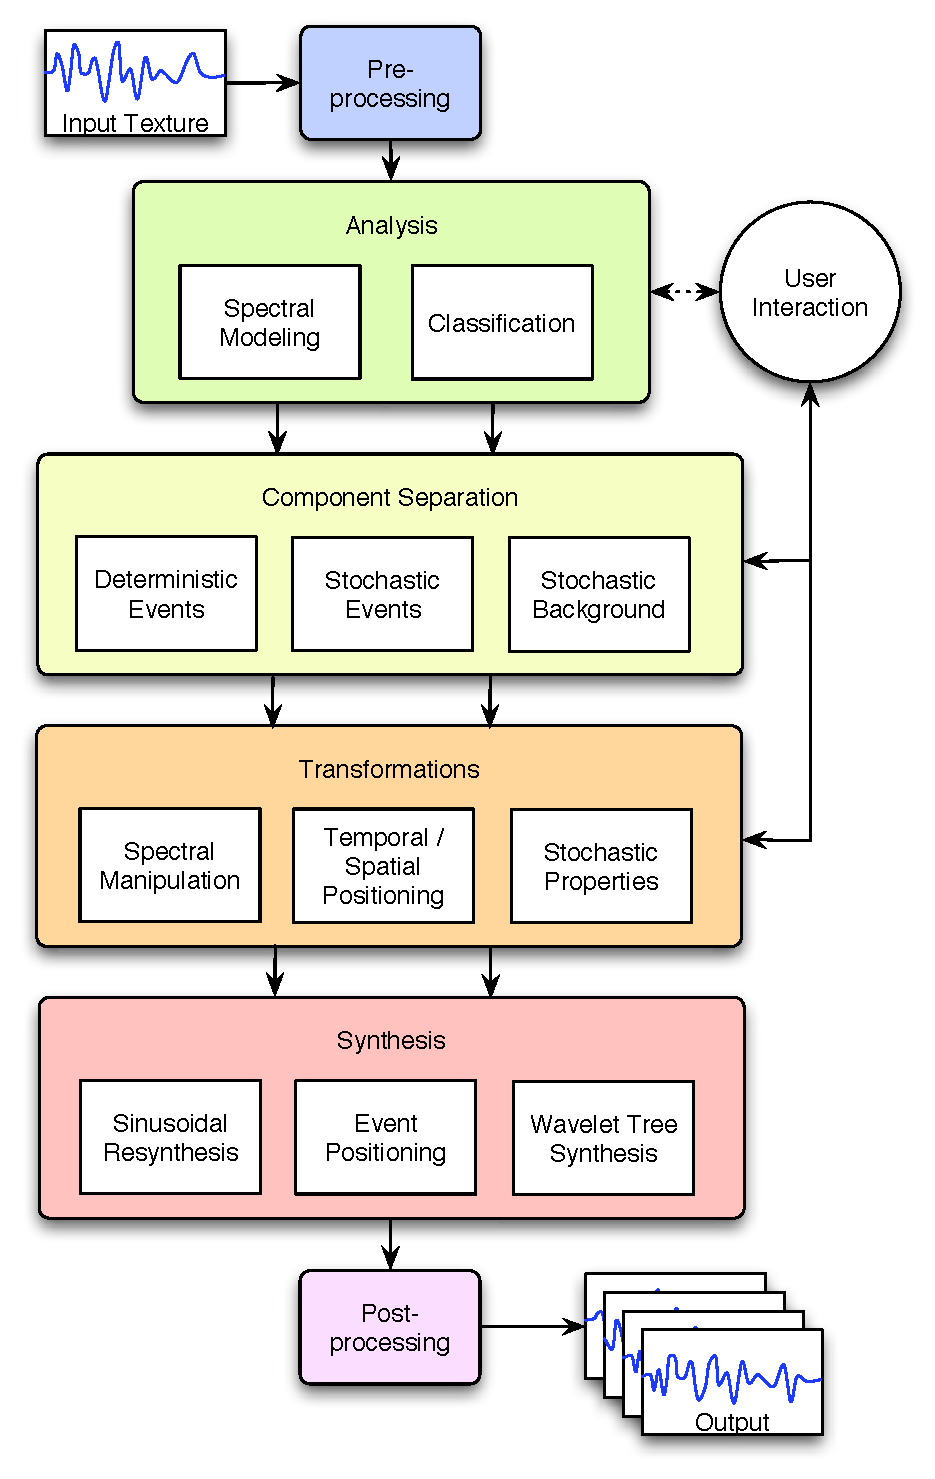
\includegraphics[width=.95\columnwidth]{ourpipeline.eps}
\caption{Our pipeline.}
\end{figure}

During transformation, the system or user parametrically specify how to 
construct and synthesize the output sound texture(s).  For foreground
events, transformations include high-fidelity frequency/magnitude-warping, 
time-stretching, and transformations that controls the temporal and spatial 
density of event instances.  For background textures, it is possible to parametrically
alter the density of the sound, as well as "similarity" to the original template.

For example, if we take the engine accelerating event template from our 
street scene, we make difference instances of the event with varying 
loudness, frequencies and durations.  We can then specify for them to occur 
according to some probability, or as a group (cars at a traffic light 
accelerating together from rest).  Furthermore, we can place each instance
"sonically" in space.  The user can experiment with each of these and 
preview the result before the final reconstruction / synthesis stage.  Transformations
on events and background are discussed in Section 5.

(TODO: need to show scripting language or user interface here or earlier)

The reconstruction / synthesis stage takes event and background templates,
and produces the output texture according to specification.
The stochastic background texture is repeatedly decomposed and 
recomposed (using wavelet tree learning and or dafxtflp) into new,
perceptually similar, non-repeating stochastic background textures, 
which are layered with the foreground of deterministic events.  From the 
original street sound template, it is possible to generate an arbitrary length 
sound texture with similar background and distribution of events.  Also, the 
loudness, frequency-content, density, and spatialization of each 
component can be controlled and modified independently.  From the same 
template, we can generate a new sound texture that gives the impression 
of many more cars and bus, or that of a sparse, quieter intersection, and 
vary the parameters dynamically to go from one to the other.

%what a messy pile of words.


%The Pipeline

%   3.1 pipeline\\
%       --- input\\
%       --- analysis, event separation\\
%       --- transformation\\
%       --- synthesis\\
%       --- output\\
%       --- control points\\
%   3.2 list of contribution\\


\section{Event Identification and Isolation}

The first step in our framework is to identify and separate the \textit{deterministic events}
from the background noise. In this context, deterministic events are the sinusoidal or pitched 
components of a sound. We separate these since listeners perceive them as distinct 
occurrences against the background of more stochastic, unpitched parts of 
the sound texture. A texture may also contain transient, non-sinusoidal events such as footsteps. Hence our event identification is based on sinusoidal 
extraction methods and on further analysis of the stochastic component (TODO: write this). 

\subsection{Preprocessing}

We are considering several ways of preprocessing the given sound 
texture to enhance deterministic and transient event extraction. One strategy is to bandpass-filter 
the sound and perform event detection separately on each subband. This 
could be useful because what is perceived as an event may differ according 
to the spectral range in which it takes place. For example, high-frequency
sounds
%(specific range?)
are easier to detect than low-frequency sounds of 
the same magnitude (I think). So processing each subband separately allows 
for better fine-tuning of the event detection / tracking parameters.

Another form of preprocessing is to intelligently segment the given sound 
texture using the MARSYAS framework. Each segment could then be processed 
separately. Since each segment is a contiguous-time clip with uniform 
features, doing this could also aid event identification.

The thing we actually do is block DC.

\subsection{Classification}

As described earlier, classification of sounds can give us hints on the 
appropriate parameters or techniques to use for event detection and 
tracking. We can classify based on various features, including power, spectral centroid and 
rollof, spectral flux, zero crossing rate, and Mel-Frequency Cepstral Coefficients. For 
domain-specific tasks, features such as Parametric Pitch Histogram, and Beat/Periodicity 
Histogram can be calculated and used. These features also aid segmentation of the original 
sound, as described in Section 4.1.

\subsection{Sinusoidal Modeling}

To identify deterministic events, we perform sinusoidal analysis based on the spectral 
modeling framework. The sound texture is divided into possibly overlapping 
frames, each of which is transformed into the frequency domain using the 
FFT and processed separately by the sinusoidal analysis framework.

%The lowest frequencies in the spectral frame are eliminated to avoid 
%artifacts from the transform and windowing.
The maximum and average 
magnitudes of the spectral frame are computed and stored. The following 
steps are then repeated until either a specified maximum number of peaks 
have been located or no more peaks are present: %(kind of ambiguous)(why?)

(1) The maximum-magnitude bin in the frame is located.\\
(2) If the ratio of its magnitude to the average magnitude of the frame is 
below a specified number, it is assumed to be noise and we deduce that no 
more peaks are present.\\
(3) If its magnitude is below a specified fraction of the stored maximum 
magnitude of the whole frame, it is not considered a peak and we deduce 
that no more peaks are present.\\
(4) Otherwise it is added as a sinusoidal peak, and the steps are repeated 
for the next highest magnitude.

Once all the peaks have been detected, we match them with the peaks from 
the previous frame. Over time this yields tracks of peaks as they shift 
slightly in frequency and magnitude from frame to frame. The matching and 
updating of tracks takes place in the following way:

(1) Each existing track from previous frames selects a current peak that is 
closest to it in frequency. (This may not work well in some cases but we 
believe it succeeds in the average scenario.) If the difference in 
frequency is above a reasonable error amount, that track is discontinued 
and the selected peak remains unmatched.\\
(2) All remaining current peaks that have not been matched to a track are 
added as new tracks, and all existing tracks that have not found a 
continuation are removed.

\begin{figure}[h]
\centering
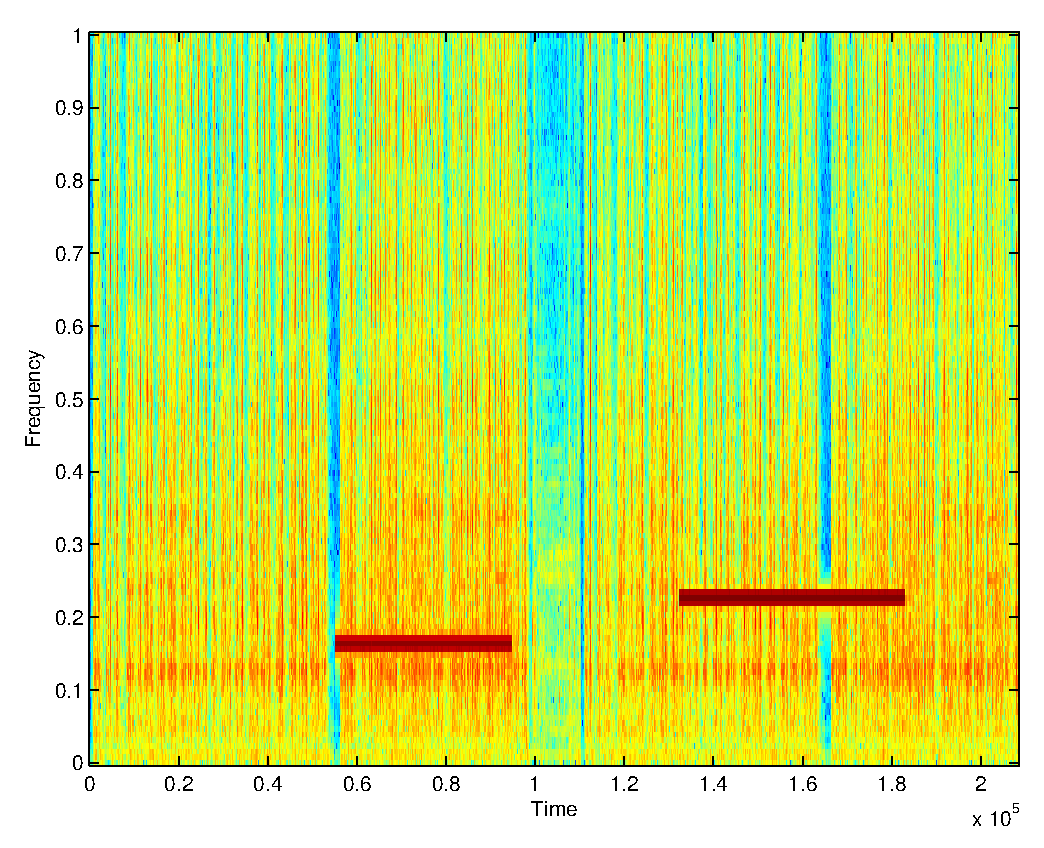
\includegraphics[width=.95\columnwidth]{story1.eps}
\caption{Sinusoids - didactic sms figure waterfall.eps}
\end{figure}

The presence of tracks makes it possible to specify that a sinuosoidal 
peak must exist across enough frames before it is accepted as an event, or 
that we can wait for a few frames before discontinuing it even if it 
vanishes temporarily. This in turn can make event representation more 
accurate/meaningful.

\subsection{Transient Detection}

This is a variant of transient dection.

\subsection{Event Representation}

Deterministic events are represented as sinusoidal tracks. For each event, we have 
access to a history of its frequency, phase and magnitude over frames, as 
well as the time of its onset, whether it is currently going on, and if 
not, the time when it ended. An extension based on this information would 
be to identify sinusoidal tracks that move in similar ways across the same 
frames, and group them as a single event or object.

Transient events are segmented and isolated sound events from the background texture.
Since they are, by definition, not captured by deterministic event isolation, they cannot be
represented as sinusoidal tracks.  Once a transient event is detected in the background
texture, it is isolated in both time and frequency range, and stored as frames of time-varying
Fourier spectra.  This representation is not as flexible as sinusoidal tracks but represents
transients better, since they tend to be more noisy than deterministic events, and is amenable
to spectral transformations.

\subsection{Residual Extraction}

The residue, or non-sinusoidal component, is extracted during the 
sinusoidal modeling. When a sinusoidal peak is discovered, the 
nearest local minima before and after the peak represent the peak's 
beginning and end respectively. We eliminate the peak from the spectrum by 
doing linear interpolation on the magnitudes of the bins between the its
beginning and end. We also randomize the phase in these 
bins.

Some artifacts still remain in the resulting residual, so an alternative 
is to segment out frames that have many, or loud, events and to extract 
the residue from the remaining frames.

% (TODO: transient event representation)

\section{Transformations}

Heading in the Transformation stage, we now have: (1) deterministic event 
templates, isolated in time and frequency from the 
background, (2) stochastic background sound texture, and (3) potential 
transient events.

During transformation, the system or user can parametrically specify how to 
construct and synthesize the output sound texture(s).  The deterministic 
events, transient events and background can be modeled and transformed 
separately.

\subsection{Event Transformations}

Since both deterministic and transient events are modeled parametrically, we can leverage 
any number of powerful SMS techniques for transformation.  They 
include high-fidelity time-stretching, frequency and magnitude warping, 
and cross synthesis. 
%(with another event or sound source - but this isn't relevant?)
Since they are represented as individual events, we also use 
probability/statistics to model the frequency of their occurence as 
well as the overall density of many instances of the same event.  
Furthermore, it is possible to spatialize event instances, giving
an impression of their respective spatial locations.  Most of these 
transformations can be applied to both deterministic and 
transient event templates.


\subsubsection{Sound Manipulation}

\textbf{Frequency/magnitude-warping} - By stretching or compressing the spectral
data, we can respectively raise or lower the frequency content, without 
affecting the duration of the sound.  For deterministic events with 
sinusoidal tracks, we only have to shift the frequencies of the tracks 
and we can do this with high fidelity for almost any factor (limited by 
our range of hearing).  For transient events, for which there is (more or 
less) only the raw spectral data, the spectrum of each will need to be 
shifted and interpolated (cite phase vocoder), and stretching by factor > 
2.0 may produce artifacts.  For any event instance, the magnitude 
(loudness) can be scaled uniformly or according to frequency.

\textbf{Time-stretching} - For events with sinusoidal tracks, we can modify the 
track's time-to-frequeny trajectory to increase or decrease the duration 
independent of the frequency.  For track-based representation, it is 
robust to change the duration by almost any factor without producing 
artifacts.  For example, (imagine that you) see figure below.  For 
transient events, a new frame-based trajectory can be computed, which 
will be overlap/added to produce time-stretching.  Once again, artifacts
are likely beyond a factor of 2.0 to 3.0.


\subsubsection{Sound Placement}

\textbf{Temporal placement} -  Explicitly place an individual event in time, or 
according to probability (need GUI or scripting language here).  It is possible
to explicitly script the occurrences of a particular event, and to apply other
transformations independently on each event instance.  It is also possible to
specify a probability distribution, such as Poisson.

\textbf{Spatial positioning} - Explicitly place (or provide trajectory for) an 
event instance in space (in world coordinates), and assign a particular 
spatialization effect by providing something similar to an impulse response
for the space.  The system can place an event instance any where in world
space (no occlusions), and calculate for distance attenuation, panning across
any number of output audio channels, and spatialization if an impulse reponse
is provided.


\subsubsection{Group Control}

\textbf{Density} - Specify density, or texture of a group of events, parameters include 
number of event instances and a probability distribution.  While it's possible to achieve
this control using temporal placement of individual event instances described previously,
this offers a more globally-aware control of a sound "crowd".  This lends to easier
control and more potential for system optimizations for a large number of sound sources,
such as in Tsingos et. al.  Also, the size of the group can be varied dynamically. 
%(ui or example)

\textbf{Spatial density} - Specify how to distribute group in space.  (need interaction here).

(TODO: this should go somewhere else): The power of the parametric model comes from the 
fact that each transformation can be applied independently of others, and each component can 
be modified independent of other event and components (such as background sound)


\subsection{Stochastic Background Transformations}

\textbf{Frequency/magnitude-warping} - Similar to transient events' frame-based 
warping - modify the frequency/magnitude of the background texture (using spectral
modeling).  This can applied either before or after the stochastic modeling.

\textbf{Time-stretching} - Slow down or speed up the background characteristics, without 
changing the pitch.

\textbf{Similarity to original sound} - Modify how similar the new generated background
will be to the original background.  A lower index of similarity will allow more randomness
in the synthesized texture.
% - by modify parameters to wavelet tree\\
%--- threshold / randomness (see below)\\
%- synthesis parameters (LPC for micro-transient)\\

%\textbf{Density}\\
% - some metric of stochastic density.\\


\section{Synthesis}

Once the sound has been separated into events and background, and the
transformation choices have been made, we can synthesize more of the sound
texture to fit the user's preferences. We synthesize the background 
component and the events separately and combine them to produce the 
final texture. By default the synthesized texture emulates the original texture as much 
as possible.
%probability model?

\subsection{Stochastic Background Generation}

The background is generated using an extension of the wavelet tree 
learning algorithm by Dubnov et. al. ~\shortcite{Dubnov02}. The sound is 
decomposed into a wavelet tree, where each node represents a wavelet 
coefficient and its depth corresponds to its resolution.  The wavelet 
coefficients are computed using the Daubechies wavelet with 5 vanishing 
moments. A new wavelet tree is then built where each node is picked 
based on the similarity of its ancestors and its first k predecessors 
(nodes at the same depth) to corresponding sequences of nodes in the 
original tree. The learning algorithm also takes into account the amount of 
randomness desired.

We added the option of incorporating randomness into the first step of 
the learning and modified k to be a fraction of the total number of 
nodes at the current depth, instead of a fixed number. We also found 
that we can avoid learning the coefficients at the highest resolutions, 
without perceptually altering the results. Since the wavelet tree is binary, every additional 
level learned approximately doubles the running time. So not learning the highest level 
decreases the running time accordingly. This optimization allowed us 
to build a real-time version of the wavelet tree analysis and synthesis. 

%(TODO: fix this)
%- wavelet tree learning works better because we have already separated out 
%what wavelet tree is not good at handling - harmonic events.

\subsection{Event Synthesis}

The deterministic events are synthesized from their representative tracks with 
sinusoidal resynthesis. We linearly interpolate frequency and magnitude 
between consecutive frames before computing the time-domain sound from 
these. 

Deterministic events can be placed in the synthesized texture according to their 
distribution in the original texture, as shown by Zhu and Wyse 
~\shortcite{Zhu04}. But the user can also request more instances of a 
certain type of event or less of another, for a customized sound 
texture.  For example, a view of the spectral domain over time shows 
distinct peaks, or events, that the user can select. If an event lasts 
long enough, it can also be synthesized and played in isolation so that 
the user can decide its role in the final texture.

Transient events can be directly mixed in to the output after all the appropriate
frequency-warping, time-stretching, and spatialization effects are applied.

%example and figure

\subsection{Putting It All Together}

The background and events are mixed. At this point the user can sit back and enjoy 
the display, or interactively fine-tune it, depending on the degree of involvement with which 
he is most at ease. Minimal involvement entails stating the parameters at a high level and 
allowing the various components to do their job. More low-level control would involve 
listening to and adjusting the synthesized components separately, and then doing the same with 
the combined sound texture. Some hybrid between these two approaches may also be possible.

\section{User Interface}

Unofficially known as abuser interface.

figure goes here.  it looks like this:

... (each dot is a track)

\section{Results}

Figure 1 describes the effect of sinusoidal separation. Figure 1(a) shows 
the spectogram of a sound texture made up of two tones (the red 
horizontal lines) played separately against the background of a typewriter 
sound. After sinusoidal analysis and resynthesis, the tones are isolated, 
as shown in the spectogram in Figure 1(b). Since the typewriter noise 
(Figure 1(c)) is stochastic, it becomes the background, although the 
individual typewriter clicks could also be interpreted and generated as 
stochastic events. Figure 1(d) is our visualization of a synthesized 
texture based on the sinusoidal separation. The synthesized typewriter 
background is similar but not identical to the original background in 
Figure 1(c). The sinusoidal events are made to occur at different time 
intervals, and last for different amounts of time. Some of them are also 
pitch-shifted.

more figures and results go here.  use imagination.

%\subsection{Implementation}
%       - architecture
\subsection{Sound Examples}
%       - classes of sound\\
Objectively describe example sounds and results. Have some figures. 

%       - put earlier: waveform at various stages of the pipeline\\
%       - (need a web page)\\
\subsection{Evaluation}
%We have not yet evaluated our method since we are still completing the 
%implementation. Primary results are promising. When we get to the 
%evaluation stage, we can judge our system based on either the "actual" 
%similarity of the synthesized texture to the original, or by their 
%perceptual similarity. The former would require identifying or defining a 
%suitable error metric, while the latter would involve designing and 
%conducting (and participating in) a user study. Since our goal is to 
%generate the sound texture that the user wants to hear, a user study is 
%important.  However, a good error metric would also be useful.
Evaluate above examples.
Shirley's idea of having someone construct a new sound texture from existing
ones and an example to replicate. %(THe souhd of slence)

%However, a good error metric would also be useful for 
%judging the psychology soundness of the users.

%However, a technical error metric would also be useful for 
%preliminary testing or for contradicting the results of the user study if 
%necessary. 

%       - error metrics\\
%       - user study\\


\section{Conclusion and Future Work}

We have described a framework for synthesizing unlimited length, perceptually-convincing 
sound textures with separate control over individual foreground events and the background.  
Given an example sound texture,  the system can automatically locate and isolate deterministic 
and stochastic events, which can then be transformed 
and placed into new sound textures as individual occurrences or in groups.  Our framework 
also allows users to interactively highlight points of interest in the sound to isolate as 
events.  The background texture is also isolated and segmented into reusable templates.  The 
separations allows for components to be transformed independently and provides a means to 
combine specific elements from completely different sound textures.

Unlike existing approaches, our framework separates a given sound into well-defined 
deterministic, transient, and stochastic components, which fundamentally allows a greater 
level of control over the variety and quality of the synthesized texture.
We also demonstrated an interactive paradigm for building new sounds textures, which include 
iterative refinement of events, interact previews of transformations, grouping, and placement 
in time and space.  Due to the separation, our system is effective in analyzing and 
synthesizing many classes of sounds (this is not true at the moment).

While our system has no fundamental restriction on the type of input sound texture to model,
there are limitations, such as when two events have overlapping spectra, it's hard for the
analysis to tell them apart.  What about events that have strong deterministic and stochastic 
components?  What about long time-scale events with complex temporal and spectral behavior?
Example: like a motorcycle? Also, foreground vocals (such as children singing/yelling) or many 
musical sounds are difficult to capture faithfully.

(TODO: future work)

\bibliographystyle{acmsiggraph}
\nocite{*}
\bibliography{template}
\end{document}
